\section{Folding crease patterns} \label{sec:folding}
In this section, we explore the different ways one can fold a given crease pattern, and derive objectives to control them.

\begin{figure} [h]
	\centering
	\includegraphics[width=0.7\linewidth]{figures/curved_fold_through_curve.pdf}
	\caption{(TODO BETTER FIG) In the future I'll place here a crease pattern and 4 different configuration for the same deformation of the curve. 2 of them will be 2 different smooth surfaces and the other two will be curved folds by picking 2 different ones from both sides. }
	\label{fig:curved_fold_through_curve}
\end{figure}

%Two intersecting developable surfaces can be flattened along their intersection if the intersected curve have the same geodesic curvature on both surfaces. 
\subsection{The smooth and combinatorial parameters of a single crease}
A single straight crease is rather boring, mathematically speaking. Straight lines can only be folded as in classical origami, i.e. by keeping them straight \cite{demaine_lens}. Hence the folding process of a single fold can be described by a single real number, representing the constant dihedral angles between the nearby planes. There are far more degrees of freedom for folding a curved crease; Up to rigid motion, a curved folding motion can locally be described by two smooth \textit{functions}: the curves' curvature $k(t) > k_g(t)$ and its torsion $\tau(t)$  \cite{more_on_paper, duncan_folded}. Indeed, let $\gamma(t)$ be a curve on a flattened crease pattern and $\Gamma(t)$ is its embedding in $\mathbb{R}^3$. Let $k(t)$ be the curvature of $\Gamma(t)$, and $k_g(t)$ the curvature of of $\gamma(t)$, i.e. the curve's geodesic curvature, such that $k_g(t) = k(t) \cos(\alpha(t))$. Assuming the curve along the surface is indeed bend such that $k(t) > k_g(t)$, then there are 2 distinct planes containing $\Gamma'(t)$ and forming an angle of $\alpha(t)$ with the curve's osculating plane. A curve folded surface is then a consistent smooth choice of a different tangent plane for each "side" of the curve, which are dependent on $k(t),\tau(t)$ (see Fig. \ref{fig:curved_fold_through_curve}). The tangent planes from both sides are reflections of one another through the osculating plane of the curve \cite{curved_folding_kilian}.
The folding angle of a curved crease can vary along the curve, and the ruling patterns can change during the deformation. The folded shape is locally not determined only by these two smooth functions as there is an additional \textit{combinatorial} degree of freedom: the choice of a surface at each side (see \figref{fig:curved_fold_through_curve}). There are four options, two of which creates discontinuity along the crease (see \figref{fig:curved_fold_through_curve}). %We call one folded configuration a mountain fold and the other a valley fold. %We follow \cite{demaine_lens} to distinguish between the two type of folded configurations by calling one choice a \textit{Mountain} fold and the other a \textit{Valley} fold. %We note that by \cite{demaine_lens}, a fold always consistently stays mountain/valley throughout the entire creased curve. Assuming a given normal orientation, a fold is said to be a mountain fold if the normal of the surface TODO:ADD EXPLANATION. 


%The curvature and torsion also dictates the ruling patterns of the developable surfaces, generally changing while folding and bending the surface. Deforming a curved crease locally determines the shape of both surfaces around it, and the exact regions of surfaces influenced by that fold depend on the ruling patterns themselves. As mentioned, the rulings patterns themselves can change which can smoothly change during the deformation itself. 

%(there's the cone singularity case where a curved fold is more local (as focused on the cone point) but I think this requires the curve to be C^1.. should mention it?

\subsection{The combinatorial parameters of multiple creases}
Curved folding is well understood locally, around a small part of a single curve, as the tangent planes along the curves are reflections of one another through the folded curve osculating plane. Understanding crease patterns globally still remains a challenge. In essence, deforming one patch propagates a global deformation of the patch on the other side of the crease, a process that depends on the ruling patterns. The ruling patterns are formed as the intersections of the tangent planes, and as mentioned the ruling patterns can smoothly change during the deformation itself. When there are multiple creases this process further propagate and dictates the shape of other patches (see \figref{fig:multiple_crease_pattern}). The process becomes more complicated when some creases intersect due to compatibility constraints (see \figref{fig:multiple_crease_pattern}, right figure). 

\begin{figure} [h]
	\centering
	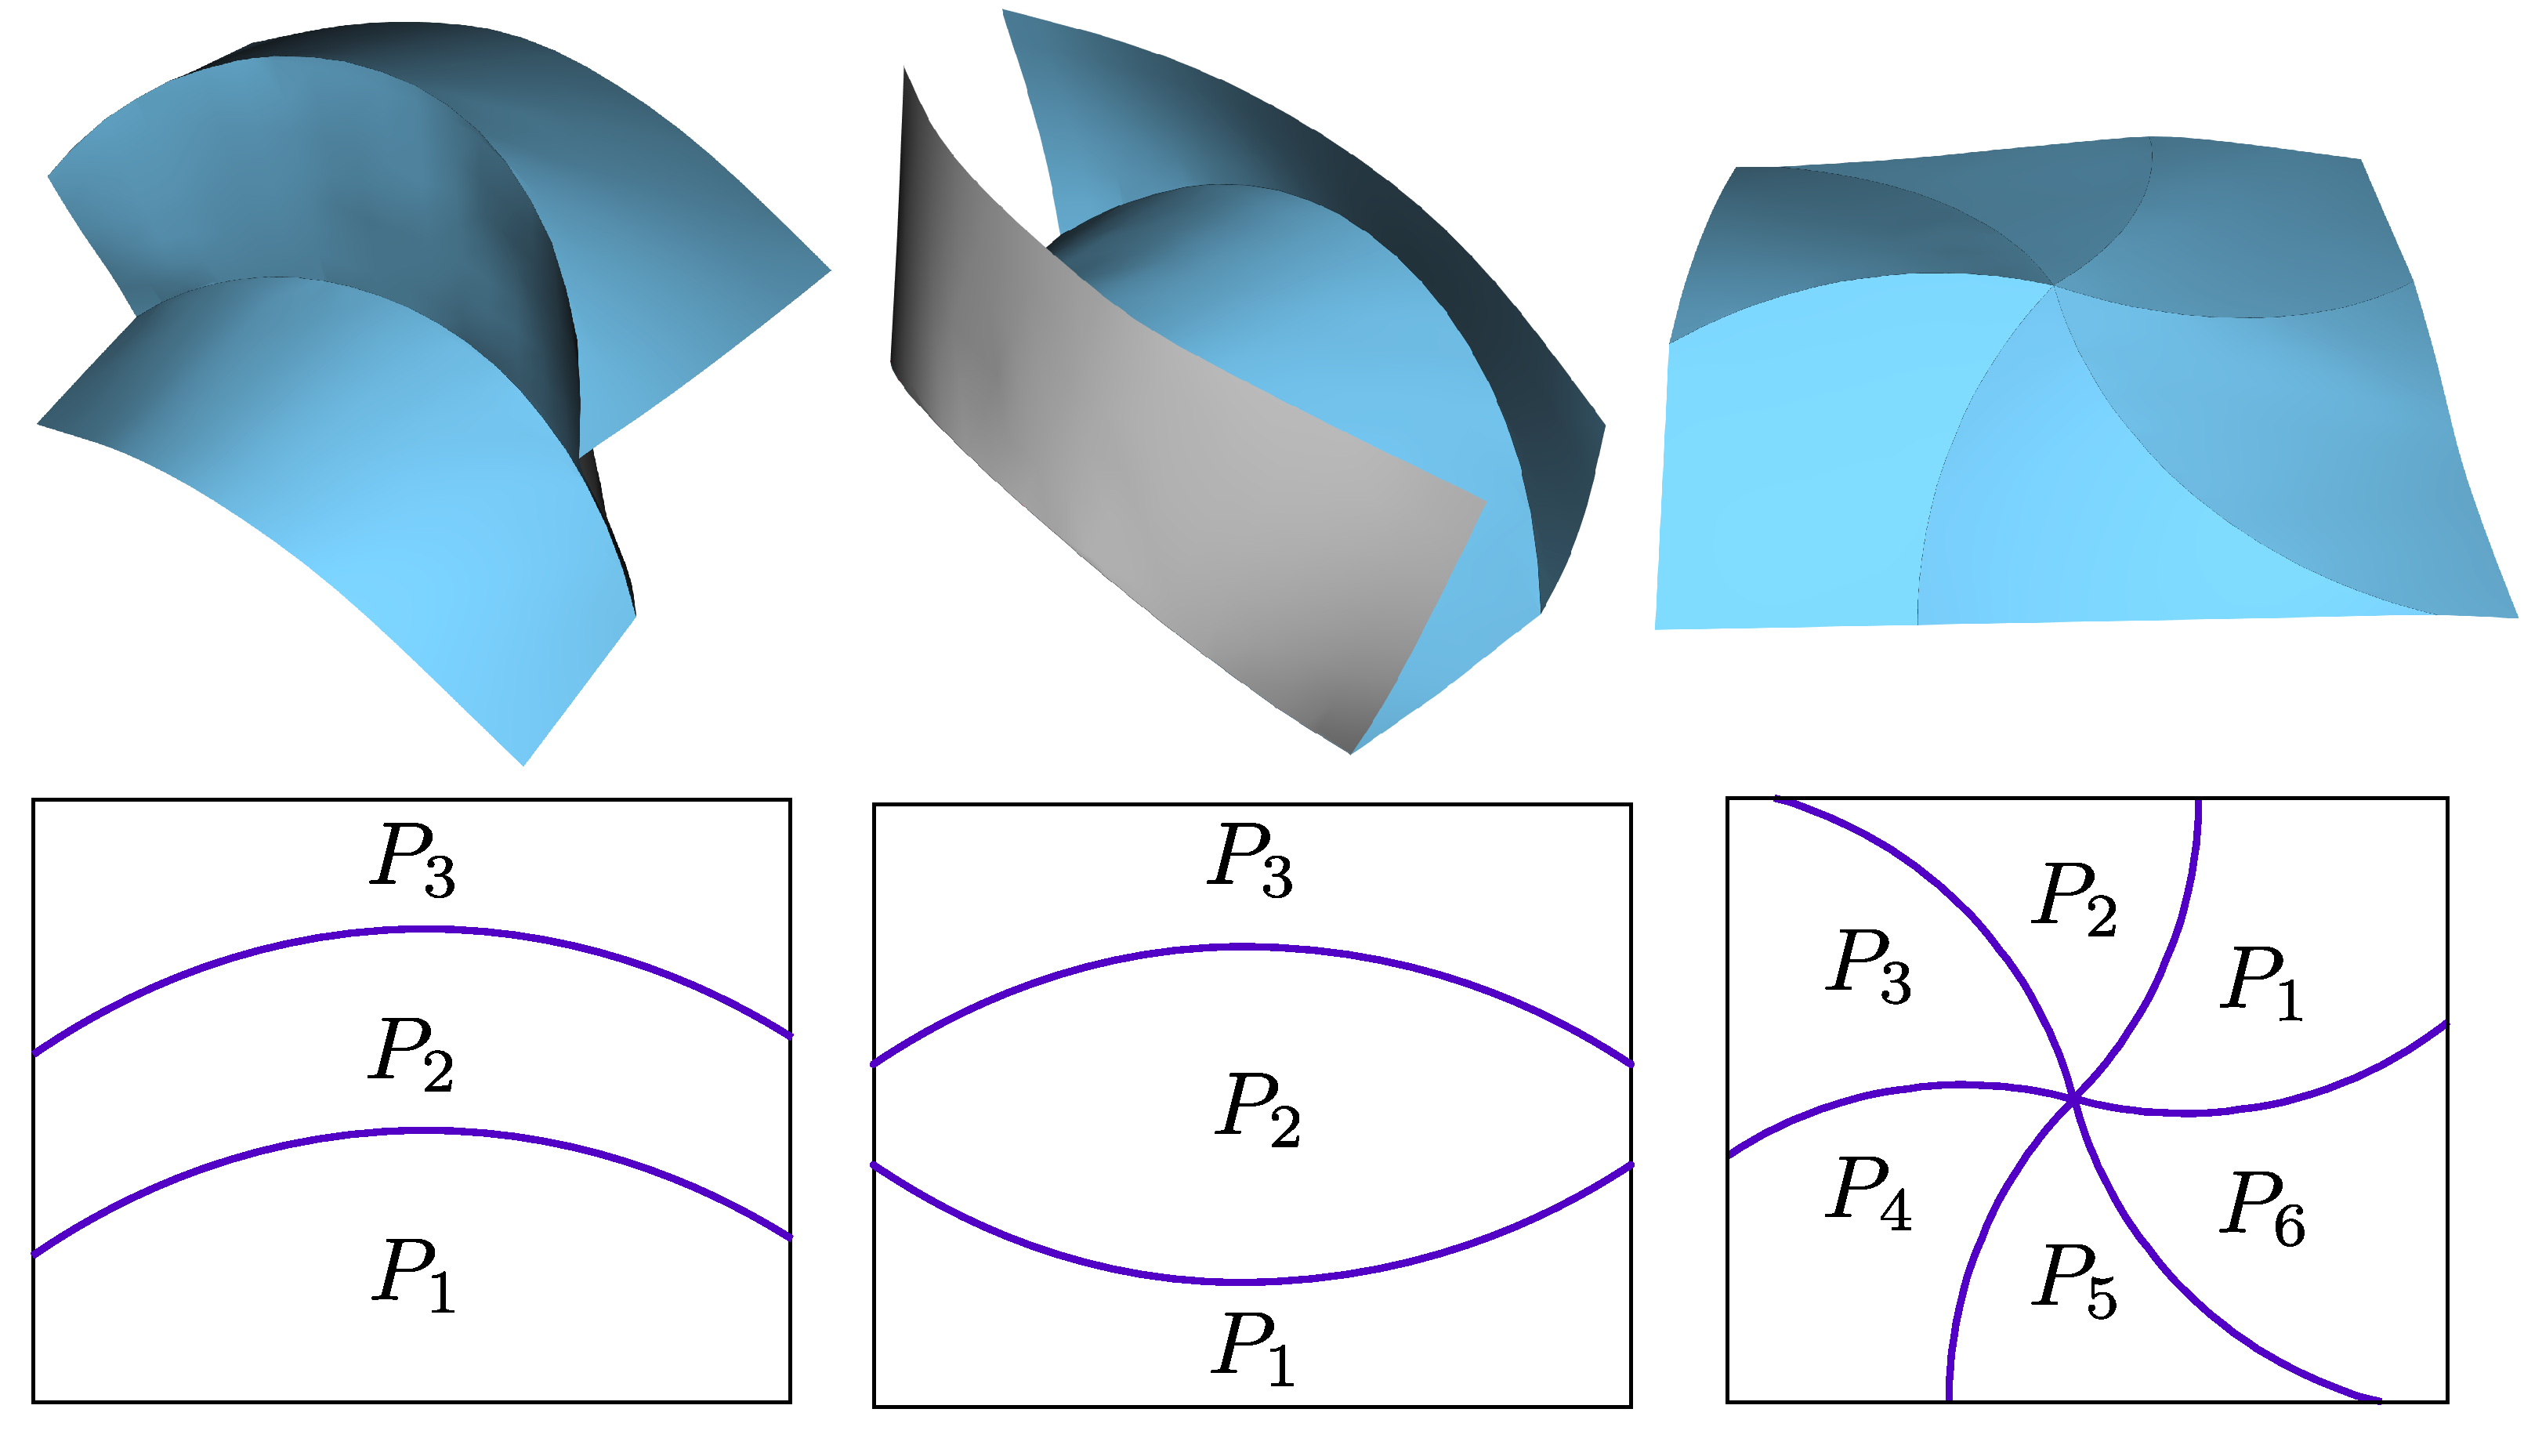
\includegraphics[width=0.7\linewidth]{figures/multiple_crease_patterns}
	\caption{Curved and straight crease patterns, decomposing a pattern into multiple components and intersecting at vertices.}
	\label{fig:multiple_crease_pattern}
\end{figure}

Generally speaking, one might be able to choose between 4 configurations of the surface at the first crease, but this choice already fixes a patch for nearby creases. The combinatorial degrees of freedom that then remain are whether each crease is folded or not (see \figref{fig:folded_and_not_folded} ). With this in mind, we note the following observation:

\begin{theorem}\label{Thm:supporting_plane}
A crease curve is folded along a given point if and only if its osculating plane at that point is locally a supporting plane for the surface (see \figref{fig:plane_side}).
\end{theorem}

\begin{figure} [h]
	\centering
	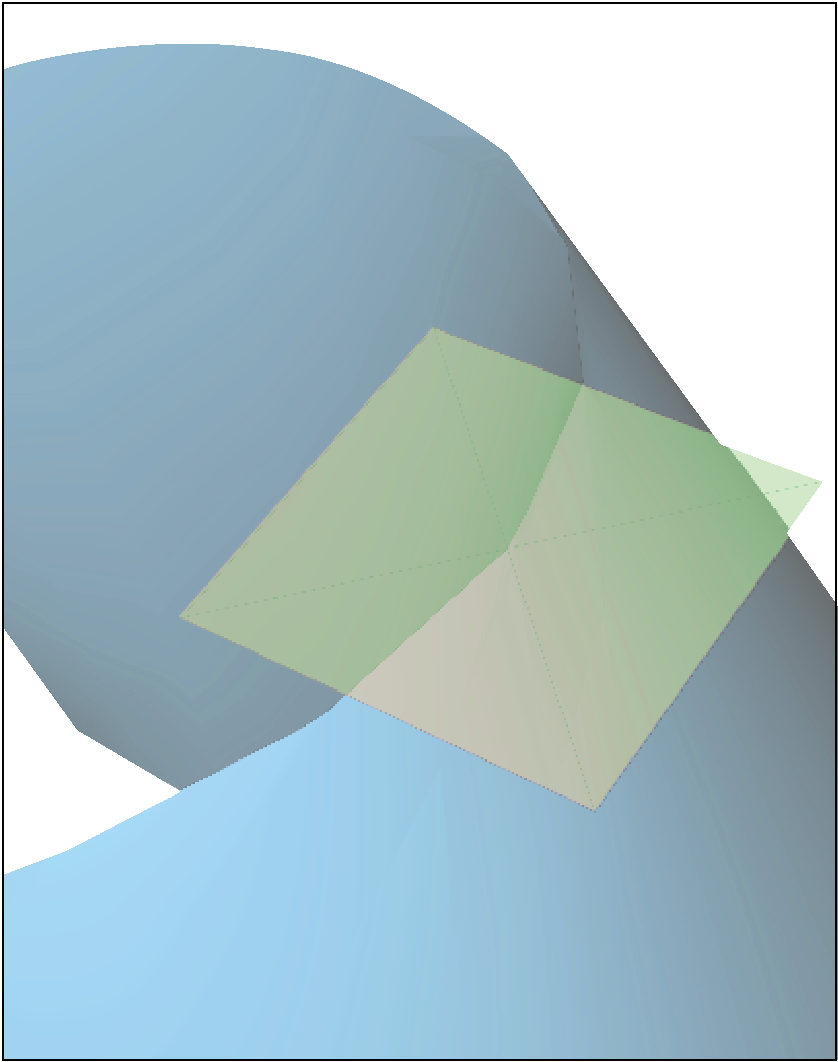
\includegraphics[width=0.5\linewidth]{figures/plane_side}
	\caption{TODO: caption and better figure}
	\label{fig:plane_side}
\end{figure}

This follows directly from the fact that the tangent planes along a crease are the same if it is smooth along it, but along a folded crease they are reflections of one another through the curve's osculating plane. As mentioned, there is often an extra combinatorial degree of freedom in choosing the type of fold, but generally only for one fold. We follow \cite{demaine_lens} to distinguish between the two type of folded configurations by calling one choice a \textit{Mountain} fold and the other a \textit{Valley} fold, distinguishing between a fold above and below the osculating plane for a given orientation. %We also note that when the curvature of the curve is not larger than its geodesic curvature, one example being a flat patch, then the tangents from both sides are the same (we should maybe call it both active and not active for that configuration?


% Motivated by homotopy stuff, we look for a function F(t). Once a crease is active, there's no need to take care of it.

% The pictures which will show are then discrete, though the smooth picture is the same. Maybe put the discrete picture in the setup as well.
% A fold is active if nearby tangents are reflections of one another, and is not active if they are the same as there is no discontinuity. (have a figure that is discrete, but explain it is also the same drawing for the smooth case).
% Write down the formula. Write down a flow. State it is inequality hence folding should be done at time = 0 when it is flat, but nevertheless a binary decision. We characterize it by the sign. 
% One can then view a folding-bending process as a smooth flow, i.e. a smooth deformation on a piecewise C^2 developable surface. The choice to make each fold active is only done during time t = 0, whereas otherwise discontinuties arise, and locally remains a curved fold as the equality.
% Problem in using it for a DOG is that we cannot hope to get it exactly. Then present binary representation. Say how it's really good (also goes to zero very fast).
% The binary characterization in the smooth case, motivate more degrees of freedom, and add the algorithm. Then add control for dihedral angles and mountain valley fold.

\subsection{Discretization}
We discretize the condition by constraining tangents formed by the orthogonal grid parameter lines to lie on one side of the curve's discrete osculating plane (see \figref{fig:osc_plane_discretization} for the notations of the edges). The edges intersecting the crease can be considered as discrete tangents originating at crease points. In the notation of \figref{fig:osc_plane_discretization}, each connected component has its own edge $e^1,e^2$ intersecting the crease. At a starting flat configuration they are the same, but a folding movement creates a discontinuity along them. We denote the tangents as $t_1 = \frac{t_1}{\|t_1\|}, t_2 = \frac{t_2}{\|t_2\|}$. We denote the curves binormal, i.e. its osculating plane's normal as $B = \frac{e_f \times e_b}{\|e_f \times e_b\|}$, noting that $e_f,e_b$ are the same along both connected components.

\begin{figure} [h]
	\centering
	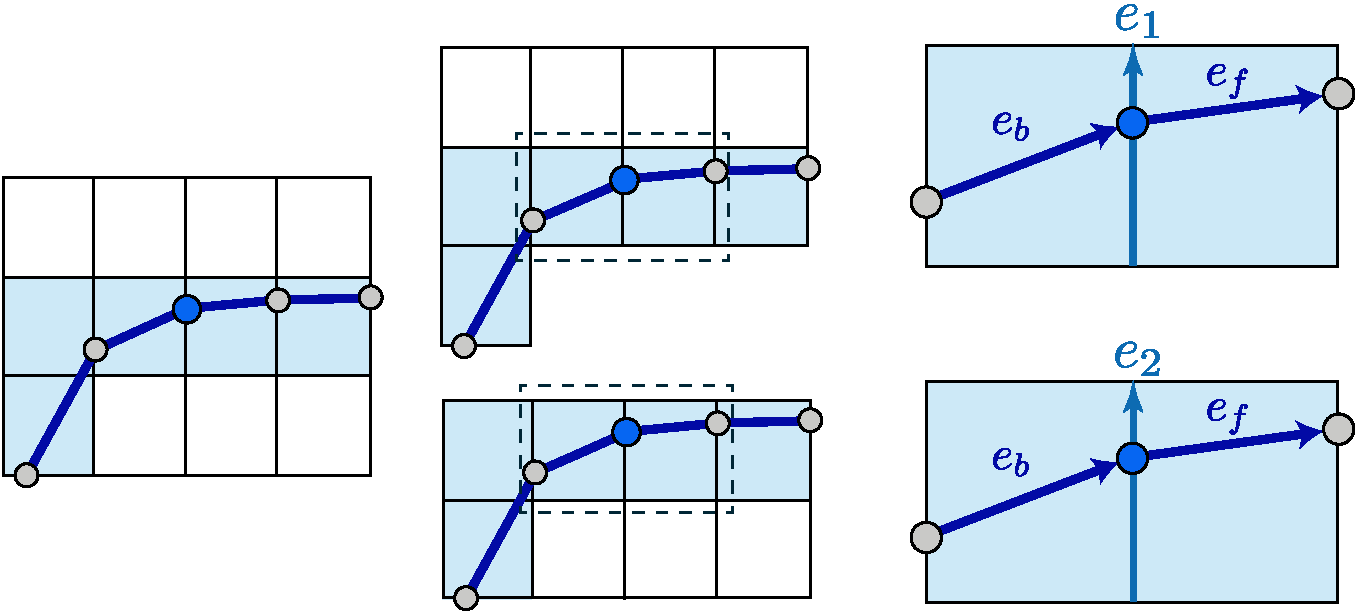
\includegraphics[width=\linewidth]{figures/osc_plane_discretization}
	\caption{Notation for edges along a crease pattern. Left: An orthogonal grid with a crease curve. Center: Following \cite{rabi2018shape}, we represent such a part by duplicating quads along the grid, creating different connected components while positionally constraining the curve edge points to match. Right: Notation for a duplicated edge intersecting the curve at the blue points ($e_1,e_2$), and the forward and backwards crease edges at the blue points ($e_f,e_b$). }
	\label{fig:osc_plane_discretization}
\end{figure}

In the notation of \figref{fig:osc_plane_discretization}, this constraint can be written as:
\begin{equation} \label{eq:folding_const_normalized} 
\text{sgn}(\langle t^1,B\rangle) +  {sgn}(\langle t^2,B\rangle) = 0
\end{equation}
with 
\begin{equation} \label{eq:sign}
\text{sgn}(x) = \left\{
     \begin{array}{@{}l@{\thinspace}l}
       -1  &: \text{if } x < 0, \\
       0 &: \text{if } x = 0, \\
       1 &: \text{if } x > 0. \\
     \end{array}
   \right.
\end{equation}
There is in fact no need to normalize the tangents and binormal directions, as the following constraint is equivalent to \eqref{eq:folding_const_normalized}:
\begin{equation} \label{eq:folding_const}
\text{sgn}(\langle e^1,e_f \times e_b \rangle) +  {sgn}(\langle e^2,e_f \times e_b\rangle) = 0
\end{equation}
\subsection{Discussion}
In the smooth case there are multiple equivalent charecterizations for a folded crease over a curved folded surface. We would like to point out some key properties of eq. \eqref{eq:folding_const}. \\
\textbf{It is suitable for homotopy based optimization methods} as it is satisfied on a flat mesh. In this sense we consider a point along a curve with zero normal curvature as both folded and not folded. \\ 
\textbf{It is minimal} and generally non-intrusive. Once a curved crease is folded on a piecewise smooth developable surface, one does not need to explicitly take extra care of folding. The discontinuity along the tangents caused by the folding means that in order for a curve to become unfolded one needs to first flatten it, and local deformations keep it folded. Conversely, a curved crease can only be folded from a flat configuration \cite{more_on_paper}. The effect of eq. \eqref{eq:folding_const} on an already-folded surface is null. \\
One could for instance distinguish curved folded with non-curved folded configurations using discontinuties along the tangents $t_1,t_2$, but lose the feasibility of the flat models. Another option to distinguish between folded and unfolded configurations is the following similar but simpler smooth constraint:
\begin{equation} \label{eq:folding_const_smooth} 
\langle t^1,B\rangle + \langle t^2,B\rangle = 0
\end{equation}
This condition is satisfied exactly in flat model. Since tangent planes along a folded creased curve are reflections of one another in the osculating plane, the condition is satisfied exactly in a piecewise smooth orthogonal geodesic net), but not on every folded piecewise DOG unless the curved crease has zero torsion, in which case folds are just folds are simply formed as a global plane reflection. Enforcing constraint \eqref{eq:folding_const_smooth} as a hard constraint is too restrictive in practice, while enforcing it as a soft constraint creates a constraint that unlike the smooth case, does not vanish once a crease is folded and hence is not minimal.

\subsection{Optimization}
We employ \theoremref{Thm:supporting_plane} and its discretization eq.\eqref{eq:folding_const} in a simple algorithm to enforce folds along creases while deforming piecewise smooth DOGs. The algorithm tries to minimize an objective, while satisfying the DOG and patches constraints as in \cite{rabi2018shape}, while also ensuring the formation of folds along crease curves.
Let $c_i$


Let $f(x)$, composed for instance as a composition of bending,isometry and positional constraints and a set of constraints $g_i(x)$ over a piecewise DOG, composed of the DOG constraints and the edge stitching constraints as in \cite{rabi2018shape}, we would like to solve the following problem while enforcing the constraints eq.\eqref{eq:folding_const} over all inner points in the crease curves.
% Say that this constraint is satisfied 
% combinatorial
% we know that as in the smooth case this only affects once, so want this to vanish afterwards
% we start feasible and we want to remain feasible as in the case of a smooth thing.
% We want to effect it as minimally as possible.
% We add a penalty method, given some energy we minimize the following
% We use them on all inner points of curves besides vertices
